\documentclass[10pt,]{article}
\usepackage{lmodern}
\usepackage{amssymb,amsmath}
\usepackage{ifxetex,ifluatex}
\usepackage{fixltx2e} % provides \textsubscript
\ifnum 0\ifxetex 1\fi\ifluatex 1\fi=0 % if pdftex
  \usepackage[T1]{fontenc}
  \usepackage[utf8]{inputenc}
\else % if luatex or xelatex
  \ifxetex
    \usepackage{mathspec}
  \else
    \usepackage{fontspec}
  \fi
  \defaultfontfeatures{Ligatures=TeX,Scale=MatchLowercase}
\fi
% use upquote if available, for straight quotes in verbatim environments
\IfFileExists{upquote.sty}{\usepackage{upquote}}{}
% use microtype if available
\IfFileExists{microtype.sty}{%
\usepackage{microtype}
\UseMicrotypeSet[protrusion]{basicmath} % disable protrusion for tt fonts
}{}
\usepackage[margin=1.0in]{geometry}
\usepackage{hyperref}
\hypersetup{unicode=true,
            pdftitle={Department Invited Speakers Do Not Reflect Trainee Diversity},
            pdfborder={0 0 0},
            breaklinks=true}
\urlstyle{same}  % don't use monospace font for urls
\usepackage{graphicx,grffile}
\makeatletter
\def\maxwidth{\ifdim\Gin@nat@width>\linewidth\linewidth\else\Gin@nat@width\fi}
\def\maxheight{\ifdim\Gin@nat@height>\textheight\textheight\else\Gin@nat@height\fi}
\makeatother
% Scale images if necessary, so that they will not overflow the page
% margins by default, and it is still possible to overwrite the defaults
% using explicit options in \includegraphics[width, height, ...]{}
\setkeys{Gin}{width=\maxwidth,height=\maxheight,keepaspectratio}
\IfFileExists{parskip.sty}{%
\usepackage{parskip}
}{% else
\setlength{\parindent}{0pt}
\setlength{\parskip}{6pt plus 2pt minus 1pt}
}
\setlength{\emergencystretch}{3em}  % prevent overfull lines
\providecommand{\tightlist}{%
  \setlength{\itemsep}{0pt}\setlength{\parskip}{0pt}}
\setcounter{secnumdepth}{0}
% Redefines (sub)paragraphs to behave more like sections
\ifx\paragraph\undefined\else
\let\oldparagraph\paragraph
\renewcommand{\paragraph}[1]{\oldparagraph{#1}\mbox{}}
\fi
\ifx\subparagraph\undefined\else
\let\oldsubparagraph\subparagraph
\renewcommand{\subparagraph}[1]{\oldsubparagraph{#1}\mbox{}}
\fi

%%% Use protect on footnotes to avoid problems with footnotes in titles
\let\rmarkdownfootnote\footnote%
\def\footnote{\protect\rmarkdownfootnote}

%%% Change title format to be more compact
\usepackage{titling}

% Create subtitle command for use in maketitle
\newcommand{\subtitle}[1]{
  \posttitle{
    \begin{center}\large#1\end{center}
    }
}

\setlength{\droptitle}{-2em}

  \title{\textbf{Department Invited Speakers Do Not Reflect Trainee Diversity}}
    \pretitle{\vspace{\droptitle}\centering\huge}
  \posttitle{\par}
    \author{}
    \preauthor{}\postauthor{}
    \date{}
    \predate{}\postdate{}
  
\usepackage{booktabs}
\usepackage{longtable}
\usepackage{array}
\usepackage{multirow}
\usepackage[table]{xcolor}
\usepackage{wrapfig}
\usepackage{float}
\usepackage{colortbl}
\usepackage{pdflscape}
\usepackage{tabu}
\usepackage{threeparttable}
\usepackage{threeparttablex}
\usepackage[normalem]{ulem}
\usepackage{makecell}
\usepackage{caption}

\usepackage{helvet} % Helvetica font
\renewcommand*\familydefault{\sfdefault} % Use the sans serif version of the font
\usepackage[T1]{fontenc}

\usepackage[none]{hyphenat}

\usepackage{setspace}
\doublespacing
\setlength{\parskip}{1em}

\usepackage{lineno}

\usepackage{pdfpages}
\floatplacement{figure}{H} % Keep the figure up top of the page

\begin{document}
\maketitle

\vspace{30mm}

Running title: Invited Speaker Diversity Does Not Reflect Trainee
Diversity

\vspace{35mm}

Ada K. Hagan, Ph.D.\({^1\dagger}\), Rebecca M. Pollet, Ph.D.\({^1}\),
and Josie Libertucci, Ph.D.\({^2\dagger}\)

\vspace{35mm}

\(\dagger\) To whom correspondence should be addressed:
\href{mailto:akhagan@umich.edu}{\nolinkurl{akhagan@umich.edu}} or
\href{mailto:libertj@mcmaster.ca}{\nolinkurl{libertj@mcmaster.ca}}

1. Department of Microbiology \& Immunology, University of Michigan, Ann
Arbor, Michigan

2. Department of Medicine, McMaster University, Hamilton, Ontario,
Canada

Figures: 1

Tables: 1

\newpage

\subsection{Conflicts of Interest}\label{conflicts-of-interest}

\vspace{40mm}

All authors affirm that there are no conflicts of interest.

\newpage

\linenumbers

\subsection{Abstract}\label{abstract}

Social role theory emphasizes the importance of ``like'' representation
to improve feelings of self-efficacy and belonging. This is an issue for
trainees in the biological sciences who are either white women or
underrepresented minorities, since there is a lack of faculty who look
like them in biology academic settings. One way to improve
representation is through invited speaker series. In this persepective,
we compare the diversity of invited speakers at one microbiology and
immunology department to the diversity of their post-Baccalaurate
trainees. We find that trainees are not proportionally represented by
the invited speakers and provide policy suggestions and tools to address
this issue.

\subsection{Keywords}\label{keywords}

inclusion, diversity, invited speakers, academia, graduate programs

\newpage

\subsection{Background}\label{background}

Long-standing systemic bias, sexism, and racism have contributed to the
underrepresentation of many racial and ethnic groups, as well as women,
in science, technology, engineering, and math (STEM) fields (NIH 2015
report, Measuring DEI 2016, (1)). Organization climate and culture that
supports inclusion of all individuals is essential to support the
retention of historically underrepresented minorities (HURM) in the
U.S., as well as non-Caucasian individuals, and women in STEM fields
(Schneider, 2013). Inclusive organization culture will not suffice in
retaining HURM, non-Caucasian individuals, and women without
organization policy changes that support their values and goals (2).

A long-standing issue within STEM fields, specifically within academia,
has been a lack of diverse representation of scientists for trainees
(graduate students and postdoctoral fellows). In order to maintain
retention of HURM, non-Caucasian individuals, and women in STEM fields,
it is important for trainees to have visual representations of
themselves as scientists. The importance of representation in retaining
a diverse group of individuals in STEM fields is supported by social
role theory (3). Individuals tend to make inferences about
characteristics that are needed to be successful in a given role by
examining individuals that most occupy that role (3, 4). Therefore,
trainees who do not see representation of themselves in senior
scientific positions, or in this case as senior faculty members, may
decide that they do not possess the characteristics that are required to
succeed. In an attempt to make science a more inclusive environment,
many individuals have attempted to address this issue by promoting the
inclusion of more women speakers at conferences (5--7). However, no
study to date has addressed invited speaker seminar series diversity
within their own institution.

Within the Department of Microbiology and Immunology at the University
of Michigan (Ann Arbor, MI, USA), each year from September to June,
faculty members have the opportunity to invite scientists from other
institutions to give a one-hour seminar in which all department members
attend. The invited seminar speaker also has the opportunity to meet
with current department faculty members and trainees. Scientists who are
invited to give seminars are widely regarded as successful and the top
in their field. Thus, if trainees are constantly being exposed to ``the
top scientist in their field'', according to social role theory, it is
imperative that the selected seminar speakers represent a diverse group
of individuals.

In this study, we examine and compare the proportion of HURM,
non-Caucasian/non-HURM, and women invited speakers to white males in the
Department of Microbiology and Immunology. Additionally, we compare
invited-speaker demographics to the current trainee demographics as a
means to gauge if trainee demographics are being represented accordingly
throughout the seminar series. Following our investigation, we proposed
a policy change to the Department of Microbiology and Immunology in how
invited speakers are selected as a means to promote inclusion in our
department and reduce stereotype threat, microaggressions, and
unconscious bias. In order to facilitate inviting a more diverse group
of scientists, we developed a set of resources that allow scientists,
within the field of microbiology, to self-identify as an HURM,
non-Caucasian/non-HURM, or a woman. These resources will promote
inclusion and diversity by providing greater representation of all
scientists and will provide hosts an opportunity to invite a more
diverse group of scientists.

\subsection{Methods}\label{methods}

Each academic year, each faculty member in the Department of
Microbiology and Immunology at the University of Michigan has the
opportunity to invite one speaker per year for a weekly seminar series.
Some of these seminar slots are dedicated to named lectureships, which
are decided by committee, and three trainee-invited speakers. We
analyzed the demographics of invited speakers and faculty hosts for five
academic years (Fall 2014 - Spring 2019), and compared them to the
current trainees when the data were analyzed (Spring 2019). Each speaker
was only counted once and those listed as departmental faculty members
or as a ``host'' at any point could not also be considered ``invited
speakers''. The list of faculty hosts was used as a proxy for faculty
demographics since as hosts, these faculty members are visible
representatives of the department. The trainees were identified using
from departmental email lists that included masters students, doctoral
students, and post-doctoral fellows.

This is a retrospective study, thus speakers were not asked for their
identities at the time of visit. Instead we hand-coded proxy
demographics using personal knowledge, photos, and CVs. The presenting
gender of each individual was assigned using a binary system
(man/woman). Due to the low number of individuals in the study,
race/ethnicity demographics were split in three groups: Caucasian,
Historically Under-represented Minority (HURM), and
Non-Caucasian/Non-HURM (NCNH), each with a binary (yes/no) possibilty.
Caucasian was assigned using the current U.S. Census definition where
those of Middle Eastern, European, and Russian descent are included.
HURM individuals were restricted to those with African-American,
Indigenous, Alaskan/Hawaian Native, Latinx and/or Hispanic heritage. All
others were placed into the NCNH group. We recognize that our proxy
demographics are a limitation of the analysis and want to acknowledge
that biological sex (male/female) is not always equivalent to the gender
that an individual presents as (man/woman), which is also distinct from
the gender(s) that an individual self-identifies as. We also want to
acknowledge that there are many other identities that are not captured
in this limited analysis.

Data were analyzed and figures generated in R Statisical Software, using
relevant packages (8--20).

\subsection{Results}\label{results}

To understand the representation of women, we compared the proportion of
women in each academic role. At the trainee level, more than half of
students and postdoctoral fellows were women. That dropped to 46.77\% of
faculty hosts and 38.73\% of the invited speakers (Fig. 1A). Of 27
lectureships over the five year period, 37.04\% were awarded to women.
The proportion of women as faculty hosts and speakers is equivalent to
global estimates that 40\% of microbiologists are women, with a slightly
lower representation of women in lectureships (21).

Our analysis identified an over-representation of Caucasian individuals
as hosting faculty and invited speakers (80\% each), relative to the
proportion of Caucasian trainees, which was 55\% (Fig. 1B). We also
observed declines in the representation of HURM and NCNH faculty and
speakers relative to the trainees (Fig 1B). HURM trainees made up 11\%
of the department, on track with the 11\% of microbiology and immunology
doctorates awarded in 2017 (22). However, only 8.5\% of invited
speakers, and none of the hosting faculty, were HURM scientists. NCNH
trainees were 34\% of department students and postdocs (22\% of
microbiology and immunology doctorates in 2017), but only 19\% of
hosting faculty and 10.5\% of invited speakers (22).

The more prestigous invited speaker lectureships were also dominated by
Caucasian scientists, who comprised 81.48\% of those awarded (Fig. 1C).
HURM and NCNH scientists were awarded 3 and 2 lectureships,
respectively. Because the intersection of identities can compound biases
and outcomes, we further examined the lectureships by gender and
race/ethnicity status. Caucasian men and women accounted for 44.44\% and
37.04\% of the lectureships, respectively. Just 18.52\% of lectureships
were held by non-Caucasian men while none were held by non-Caucasian
women (Fig. 1D).

\subsection{Discussion}\label{discussion}

{[}Add paragraph summarizing findings {]} According to social role
theory, this department is not adequately serving their non-Caucasian
trainees.

Several papers have investigated the representation of women at
scientific conferences, however, we have only identified one that
focused on invited speakers at universities (23). In their study,
Nittrouer et al, examined 3,652 talks at 50 U.S. institutions in 2013 -
2014 and found that women faculty are less likely to be invited
speakers, despite similar acceptance rates. These results suggest that
women faculty are less often invited as speakers. We have not been able
to identify any other publications examining scientific speaker
diversity beyond gender. This seems to be the first. This is concerning
since conclusions drawn from gender-based studies are often framed, and
considered, to be applicable to other marginalized groups (e.g., HURM).
This is a flawed assumption. While there is no doubt some overlap, each
group remains marginalized due to a unique complex set of factors that
cannot always be solved by gender-based solutions. US-serving
institutions, such as the University of Michigan have a particular
responsibility to the historically suppressed populations included in
our definition of HURMs. We therefore implore US institutions to apply
this framing to their discussions and research.

Departments have different processes and criteria for selecting invited
speakers, but it is a matter of pride to bring the best scientists
possible. It may be that the definition of ``best'' poses a problem to
women, who need three-times as many publications as their men colleges
to be considered equally competent (24), and those that identify as HURM
and Asian, who report having to work harder than white men to be
perceived as legitimate scholars (25). Some departments only invite
tenured faculty, which severely limits the number of potential speakers
who are white women or non-Caucasian. Yet, another scenario is that
pre-tenure faculty members invite prestigious, tenured faculty in their
field to network and secure letters for their own tenure package. The
increased burden of white women and non-Caucasian scientists to prove
competency decreases their likelihood to be considered for either tenure
or as possible source of tenure letters.

Each underrepresented group in our cohort faces a complex set of
barriers to achieving faculty status. For instance, the decision to
invite a woman may also be negatively impacted by assumptions about
competency and dedication. The dedication of women who have children to
their work is perceived to be less than that of their colleagues, i.e.,
men who also have children (26--28). The perceived prioritization and
commitments of women to family over work may cause faculty to doubt
their acceptance of a speaking invitation, despite the prestigious
nature of these invitations and evidence that men and women accept at
similar rates ({\textbf{???}}, 23). As a result, the faculty member
invites a different colleague who they feel is more likely to agree (and
is a man). Another large portion of our sample were the NCNH cohort, who
are predominately Asian/Asian American individuals. Although Asian
scientists are well-represented in the US scientific workforce, they
face significant bias and barriers to inclusion in society and academia
(29, 30). For instance, despite the higher employment rate of Asian
scientists, they were not well-represented in the more prestigious
lectureships.

While HURM and NCNH share some experiences, differences including
varying rates of hiring and tenure promotion mean unique considerations
are important for inclusion of each group (31). For instance, a major
barrier to inclusion of HURM faculty at similar proportions to HURM
trainees is the low transition rate of scientists from HURM backgrounds
to faculty positions and the associated low proportion of HURM faculty
(32). The proportion of HURM faculty at the Assistant and Associate
Professor level is currently higher than at Full Professor so it will be
difficult to increase speaker diversity if early-career researchers are
not being considered (33). Increased performance expectations and
patterns of exclusions are consistent themes in studies characterizing
the HURM faculty experience (34, 35). Therefore, inclusion of HURM
faculty in seminar series is likely essential to increasing the number
of HURM Associate and Full Professors. Even when HURM speaker rates
match the proportion of HURM faculty employment, HURM trainees will be
represented at a significantly higher proportion. Inclusion of HURM
faculty in these seminarseries is just one aspect of larger
institutional change that is needed (36).

\subsection{Instituting policy change within the Department of
Microbiology and
Immunology}\label{instituting-policy-change-within-the-department-of-microbiology-and-immunology}

In an attempt to promote inclusion within the Dept. M\&I these data were
presented to faculty members and the dept chair (Harry Mobley). Since,
trainee demographics were not represented within seminar speaker
demographics over the past 5 years, we proposed a policy change as to
how seminar speakers were being invited. This policy change included
switching from PI invited to lab invited in an attempt to allow trainees
to choose a speaker that best represented themselves.

Implict biases that affect perceptions of marginalized groups are the
primary issue, but we must acknowledge that it is not always possible to
identify members of historically under-served communities. For instance,
after data analysis, we learned that at least one speaker in our data
set should have been categorized as a HURM instead of Caucasian, but it
wasn't readily apparent from their internet presence or CV. This
limitation makes two important points: that percieved identity often
plays a larger role than self-identification, and that we need better
tools to identify members of marginalized groups. So in addition to our
policy change, we also created resources that allow scientists to
self-identify and provide host faculty with more diverse choices.

\subsection{Building Diversify}\label{building-diversify}

To help address this issue, we make some suggestions (Table 1) and have
developed a resource to identify scientists who are members of
marginalized and/or historically under-served groups. Motivated by a
lack of such resources and inspired by similar resources--DiversifyEEB
and DiversifyChemistry--we created DiversifyMicrobiology and
DiversifyImmunology. These resources are a tool for symposium
organziers, award committees, search committees and other scientists to
identify individuals to diversify their pools. Additionally, we have
built these as a tool for use by other fields and organizations to
create their own lists. Since these lists are compiled by
self-nomination, we can ensure that only scientists comfortable
revealing their marginalized identities are included.

The self-nomination form is a Google Form with entries logged in a
private Google Sheet. This form is embedded within the website and can
be linked to directly. The use of a Google Forms allows us to maintain
this database at no cost and gives us the flexibility to add questions
or change response options without disrupting previous responses.
Entries are logged in a private spreadsheet so that entries can be
screened before being added to the public database. This screening
includes two steps: confirming that each person is listed in the
database only once and that any submitted website is a personal,
professional website. If both criteria are met, a new entry is added to
the public database spreadsheet. If a person is already listed in the
database, their information is updated to the most recent submission.

This public spreadsheet is embedded in the website and can be open
separately as a locked (uneditable) Google Sheet, allowing the list to
be easily searched. We have chosen to list individuals' academic
information first in the spreadsheet to encourage a focus on academic
achievement rather than tokenization of marginalized identities.
Currently the database lists individuals in order of self-nomination but
future versions will be re-sorted based on name and/or academic field to
varying the individuals who may receive more attention for simply being
at the top of the list.

The website provides an interface to the Google forms and spreadsheets
with template pages for viewing the list, adding a name to the list, and
finding additional resources. Importantly, our website creation tool is
hosted for free by GitHub, which provides a free website for each GitHub
organization. Basic tools and skills required to set up a Diversify site
include knowledge of, or experience with, the version control tool git,
the webtool GitHub, and a text editor. A tutorial in the
DiversifyMicrobiology repository on GitHub provides links to these
resources and instructions for adapting the tool to your own field.

\subsection{Conclusion}\label{conclusion}

To increase the retention of white women and HURMS in STEM, they must
also be represented as experts. However, the invited speaker diversity
at one department does not represent the diversity of trainees. There is
a lack of research on invited speakers examining factors other than
gender. To facilite the identification and recruitment of individuals in
these historically under-served groups, we have built a tool to create
self-nominated, field-specific lists.

\subsection{Acknowledgements}\label{acknowledgements}

We thank Drs. Beth Moore and Harry Mobley and the Department of
Microbiology \& Immunology, University of Michigan for their input and
financial support that enabled publication of our manuscript. We would
also like to acknowledge Nick Lesniak and Dr.~Ariangela Kozick for their
comments and suggestions.

\subsection{Author Contributions}\label{author-contributions}

A.K.H. collected the data, assigned demographics, analyzed the data, and
created the website. R.M.P. created the Google lists, forms, and website
content and the description of their maintenance. J.L. wrote the
introduction and provided conceptual advice. A.K.H. and J.L facilited
the policy change to the UM Department of Microbiology and Immunology.
All authors contributed to preparing the final manuscript.

\subsection{Code and data
availability}\label{code-and-data-availability}

The anonymized data, code for all analysis steps, and an Rmarkdown
version of this manuscript is available at
\url{https://github.com/akhagan/Hagan_SpeakerDiversity_XXXX_2019/}.
Template and complete instructions for generating a field-specific
Diversity website are available at
\url{https://github.com/diversifymicrobiology/DiversifyMicrobiology.github.io/}.

\newpage

\begin{center}
\captionof{table}{List of suggestions and resources to increase invited speaker diversity.}
\small
\begin{tabular}{|l|l|l|}
\hline

\rowcolor{lightgray}
\textbf{Suggestion} & \textbf{Description} & \textbf{Resource} \\ \hline

Lab-invited speakers & \makecell[l]{Faculty members can request \\suggestions from trainees} & \\ \hline

Use a list & \makecell[l]{Many lists of scientists from \\under-represented and underserved \\groups are available} &  \makecell[l]{https://DiversifyMicrobiology.\\github.io/resources}\\ \hline

Create a list & \makecell[l]{Use the GitHub template \\ create a self-nomination list and \\resource for your field} & \makecell[l]{https://github.com/diversifymicrobiology/\\DiversifyMicrobiology.github.io} \\ \hline

Highlight the journey & \makecell[l]{Invite all speakers to spend \\a few moments describing their \\personal science journey} & \\ \hline

\end{tabular}
\end{center}

\begin{figure}
\centering
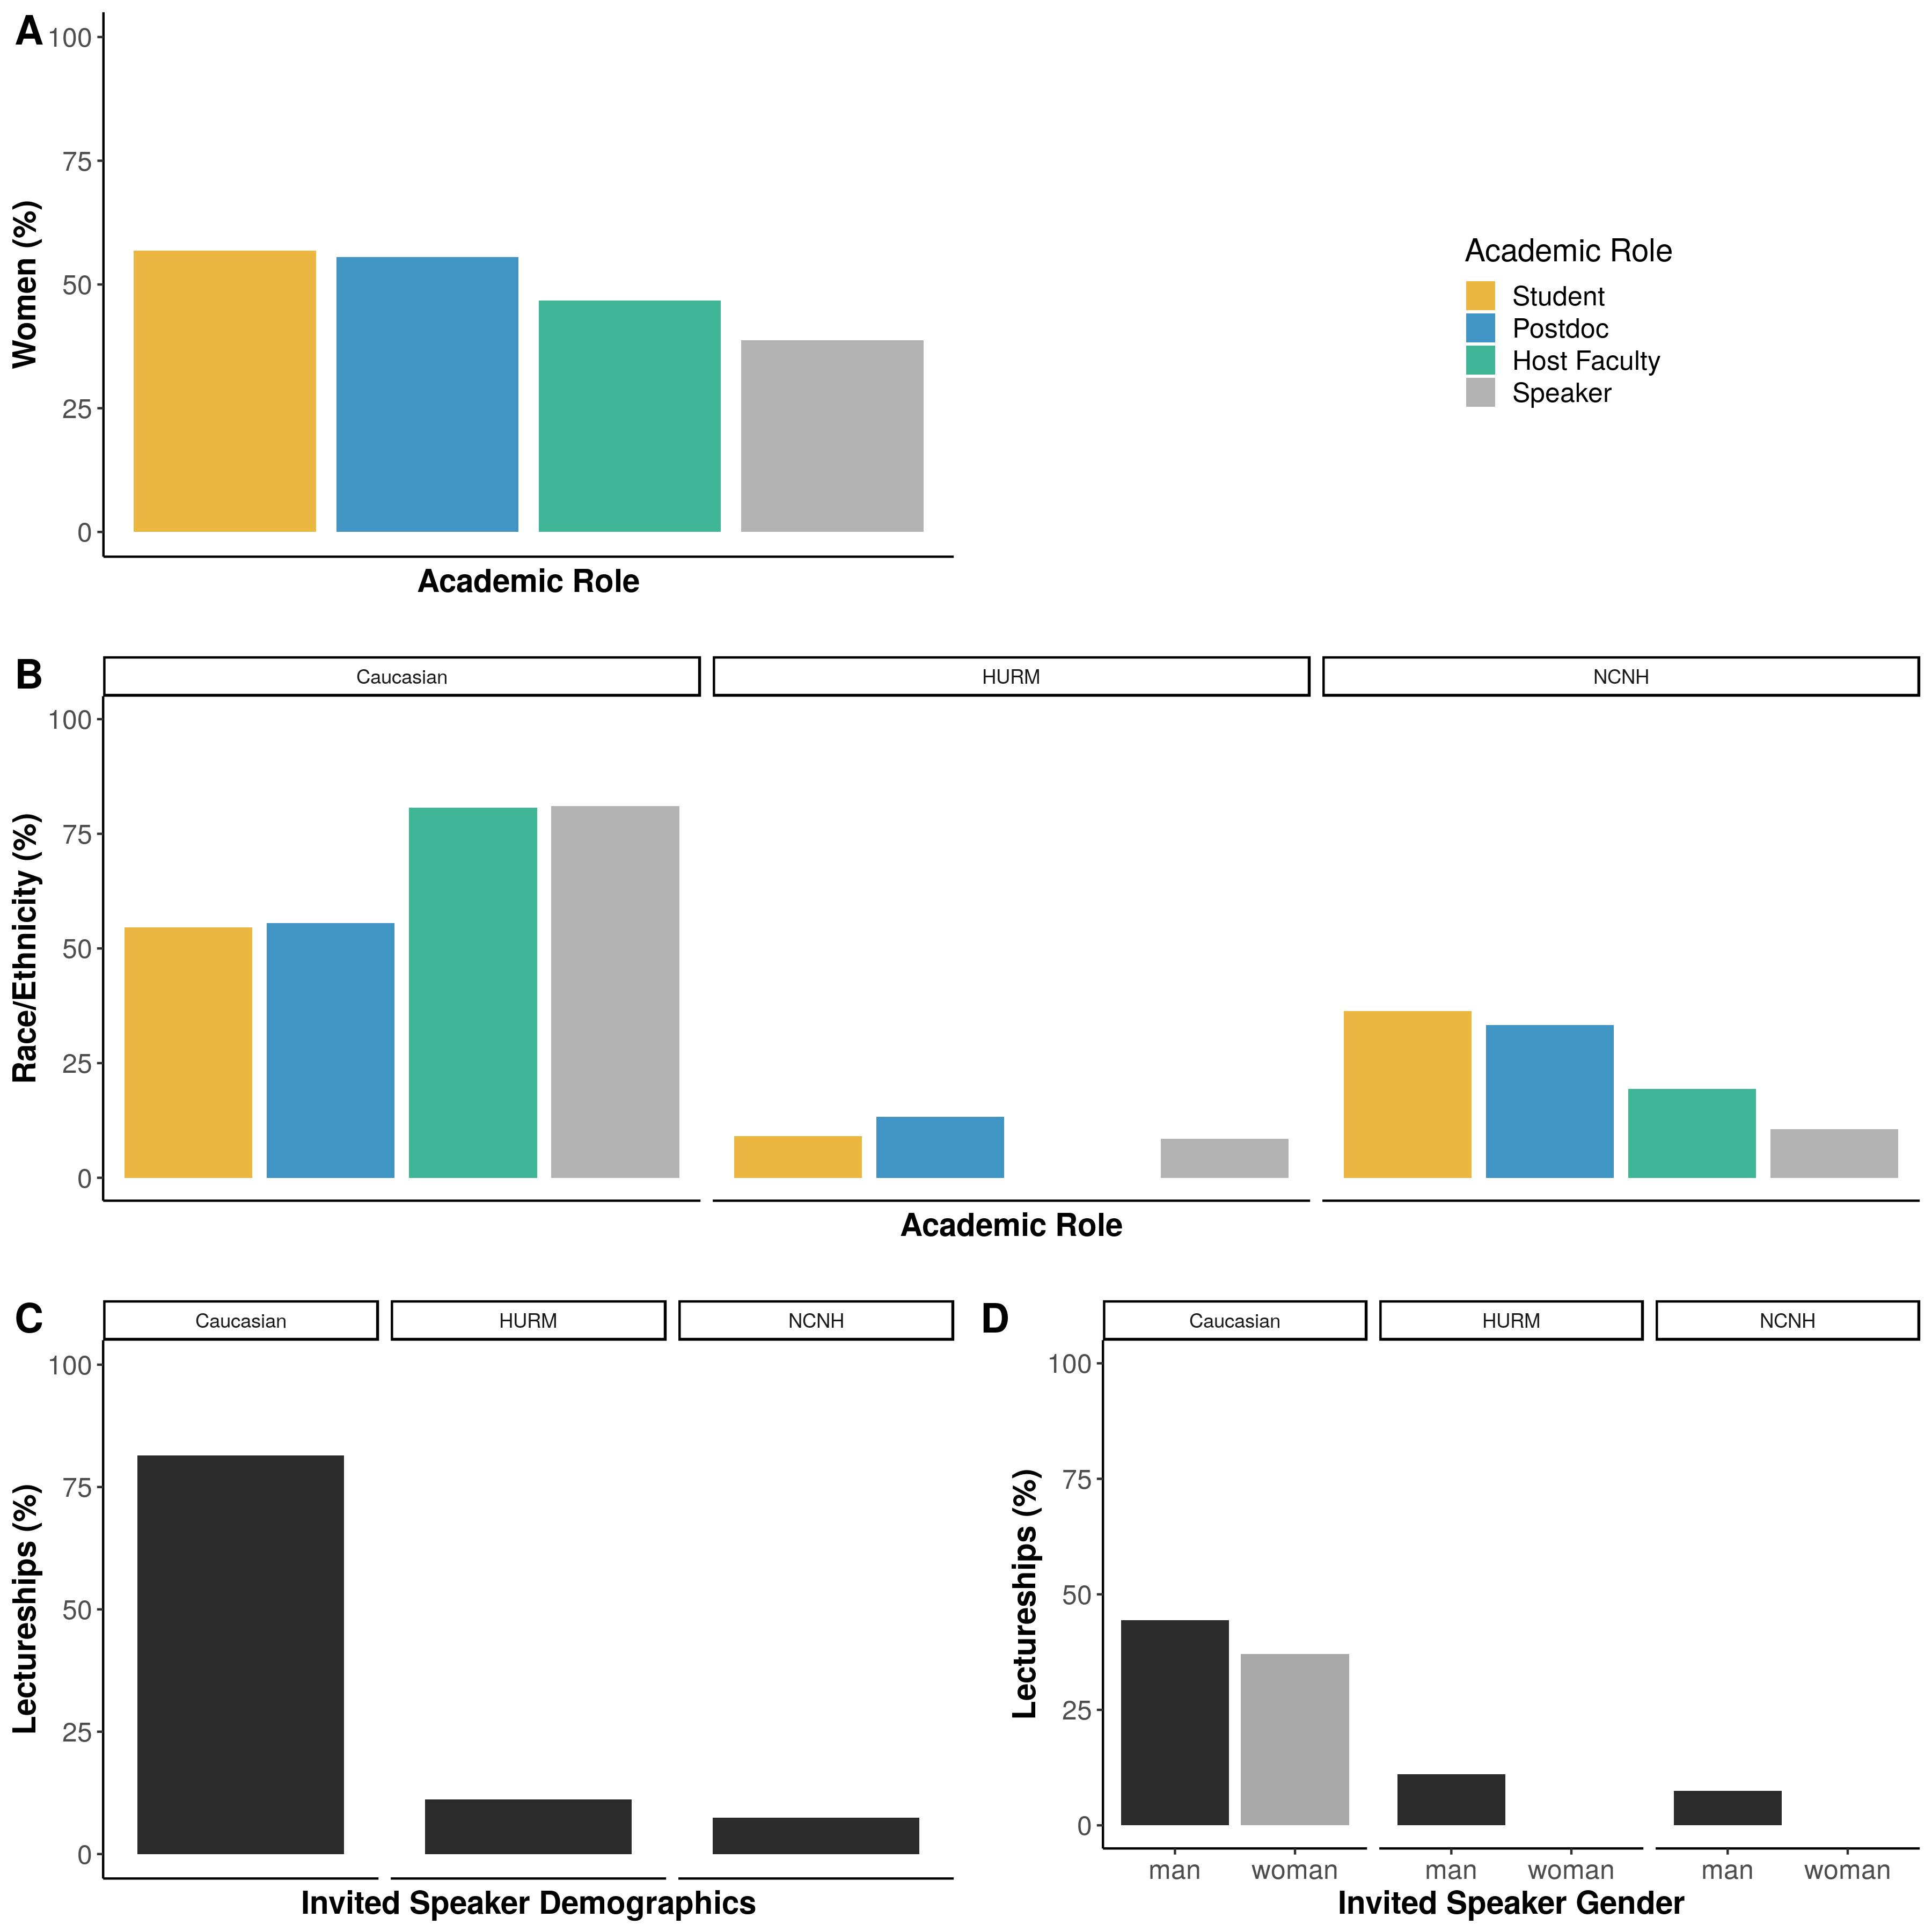
\includegraphics{Figure_1.png}
\caption{\textbf{The demographics of invited speakers, hosting faculty,
and trainees.} A) The proportion of women in each academic role. B) The
proportion of each academic role represented by individuals that are
Caucasian (left), Historically Underrepresented Minorities (HURM,
center) or International (right). C-D)The percent of lectureships
awarded to individuals that are C) Caucasian, HURM, International or D)
Caucasian or Non-Caucasian by gender.}
\end{figure}

\newpage

\subsection{References}\label{references}

\hypertarget{refs}{}
\hypertarget{ref-colloquy_2012}{}
1. 2012. Colloquy on minority males in science, technology, engineering,
and mathematics. National Academies Press.

\hypertarget{ref-Coe2019}{}
2. \textbf{Coe IR}, \textbf{Wiley R}, \textbf{Bekker L-G}. 2019.
Organisational best practices towards gender equality in science and
medicine. The Lancet \textbf{393}:587--593.
doi:\href{https://doi.org/10.1016/s0140-6736(18)33188-x}{10.1016/s0140-6736(18)33188-x}.

\hypertarget{ref-Eagly1984}{}
3. \textbf{Eagly AH}, \textbf{Steffen VJ}. 1984. Gender stereotypes stem
from the distribution of women and men into social roles. Journal of
Personality and Social Psychology \textbf{46}:735--754.
doi:\href{https://doi.org/10.1037/0022-3514.46.4.735}{10.1037/0022-3514.46.4.735}.

\hypertarget{ref-Carter2018}{}
4. \textbf{Carter AJ}, \textbf{Croft A}, \textbf{Lukas D},
\textbf{Sandstrom GM}. 2018. Women's visibility in academic seminars:
Women ask fewer questions than men. PLOS ONE \textbf{13}:e0202743.
doi:\href{https://doi.org/10.1371/journal.pone.0202743}{10.1371/journal.pone.0202743}.

\hypertarget{ref-kalejta_gender_2017}{}
5. \textbf{Kalejta RF}, \textbf{Palmenberg AC}. 2017. Gender Parity
Trends for Invited Speakers at Four Prominent Virology Conference
Series. Journal of Virology \textbf{91}.
doi:\href{https://doi.org/10.1128/JVI.00739-17}{10.1128/JVI.00739-17}.

\hypertarget{ref-casadevall_presence_2014}{}
6. \textbf{Casadevall A}, \textbf{Handelsman J}. 2014. The Presence of
Female Conveners Correlates with a Higher Proportion of Female Speakers
at Scientific Symposia. mBio \textbf{5}.
doi:\href{https://doi.org/10.1128/mBio.00846-13}{10.1128/mBio.00846-13}.

\hypertarget{ref-klein_speaking_2017}{}
7. \textbf{Klein RS}, \textbf{Voskuhl R}, \textbf{Segal BM},
\textbf{Dittel BN}, \textbf{Lane TE}, \textbf{Bethea JR}, \textbf{Carson
MJ}, \textbf{Colton C}, \textbf{Rosi S}, \textbf{Anderson A},
\textbf{Piccio L}, \textbf{Goverman JM}, \textbf{Benveniste EN},
\textbf{Brown MA}, \textbf{Tiwari-Woodruff SK}, \textbf{Harris TH},
\textbf{Cross AH}. 2017. Speaking out about gender imbalance in invited
speakers improves diversity. Nature Immunology \textbf{18}:475--478.
doi:\href{https://doi.org/10.1038/ni.3707}{10.1038/ni.3707}.

\hypertarget{ref-R_software_2017}{}
8. \textbf{R Core Team}. 2017. R: A language and environment for
statistical computing. R Foundation for Statistical Computing, Vienna,
Austria.

\hypertarget{ref-wickham_tidyverse_2017}{}
9. \textbf{Wickham H}. 2017. Tidyverse: Easily Install and Load the
'Tidyverse'.

\hypertarget{ref-cowplot}{}
10. \textbf{Wilke CO}. 2019. Cowplot: Streamlined plot theme and plot
annotations for 'ggplot2'.

\hypertarget{ref-markdown}{}
11. \textbf{Allaire J}, \textbf{Horner J}, \textbf{Xie Y}, \textbf{Marti
V}, \textbf{Porte N}. 2018. Markdown: 'Markdown' rendering for r.

\hypertarget{ref-rmd_book}{}
12. \textbf{Xie Y}, \textbf{Allaire J}, \textbf{Grolemund G}. 2018. R
markdown: The definitive guide. Chapman; Hall/CRC, Boca Raton, Florida.

\hypertarget{ref-rmd_rstudio}{}
13. \textbf{Allaire J}, \textbf{Xie Y}, \textbf{McPherson J},
\textbf{Luraschi J}, \textbf{Ushey K}, \textbf{Atkins A},
\textbf{Wickham H}, \textbf{Cheng J}, \textbf{Chang W}, \textbf{Iannone
R}. 2018. Rmarkdown: Dynamic documents for r.

\hypertarget{ref-knitr_2014}{}
14. \textbf{Xie Y}. 2014. Knitr: A comprehensive tool for reproducible
research in R. \emph{In} Stodden, V, Leisch, F, Peng, RD (eds.),
Implementing reproducible computational research. Chapman; Hall/CRC.

\hypertarget{ref-knitr_2018}{}
15. \textbf{Xie Y}. 2018. Knitr: A general-purpose package for dynamic
report generation in r.

\hypertarget{ref-lubridate}{}
16. \textbf{Grolemund G}, \textbf{Wickham H}. 2011. Dates and times made
easy with lubridate. Journal of Statistical Software \textbf{40}:1--25.

\hypertarget{ref-readxl}{}
17. \textbf{Wickham H}, \textbf{Bryan J}. 2018. Readxl: Read excel
files.

\hypertarget{ref-pdftools}{}
18. \textbf{Ooms J}. 2019. Pdftools: Text extraction, rendering and
converting of pdf documents.

\hypertarget{ref-wickham_scales_2018}{}
19. \textbf{Wickham H}. 2018. Scales: Scale Functions for Visualization.

\hypertarget{ref-neuwirth_rcolorbrewer_2014}{}
20. \textbf{Neuwirth E}. 2014. RColorBrewer: ColorBrewer Palettes.

\hypertarget{ref-allagnat_gender_2017}{}
21. \textbf{Allagnat L}, \textbf{Berghmans S}, \textbf{Falk-Krzesinski
HJ}, \textbf{Hanafi S}, \textbf{Herbert R}, \textbf{Huggett S},
\textbf{Tobin S}. 2017. Gender in the global research landscape.

\hypertarget{ref-nsf_survey_2017}{}
22. \textbf{Science and Engineering Statistics NC for}. 2017. Survey of
Doctorate Recipients, Survey Year 2017. National Science Foundation,
Alexandria, VA.

\hypertarget{ref-nittrouer_gender_2018}{}
23. \textbf{Nittrouer CL}, \textbf{Hebl MR}, \textbf{Ashburn-Nardo L},
\textbf{Trump-Steele RCE}, \textbf{Lane DM}, \textbf{Valian V}. 2018.
Gender disparities in colloquium speakers at top universities.
Proceedings of the National Academy of Sciences \textbf{115}:104--108.
doi:\href{https://doi.org/10.1073/pnas.1708414115}{10.1073/pnas.1708414115}.

\hypertarget{ref-BlairLoy2017}{}
24. \textbf{Blair-Loy M}, \textbf{Rogers L}, \textbf{Glaser D},
\textbf{Wong Y}, \textbf{Abraham D}, \textbf{Cosman P}. 2017. Gender in
engineering departments: Are there gender differences in interruptions
of academic job talks? Social Sciences \textbf{6}:29.
doi:\href{https://doi.org/10.3390/socsci6010029}{10.3390/socsci6010029}.

\hypertarget{ref-noauthor_seeking_2013}{}
25. 2013. Seeking Solutions: Maximizing American Talent by Advancing
Women of Color in Academia: Summary of a Conference. National Academies
Press, Washington, D.C.

\hypertarget{ref-Firth1982}{}
26. \textbf{Firth M}. 1982. Sex discrimination in job opportunities for
women. Sex Roles \textbf{8}:891--901.
doi:\href{https://doi.org/10.1007/bf00287858}{10.1007/bf00287858}.

\hypertarget{ref-Correll2007}{}
27. \textbf{Correll SJ}, \textbf{Benard S}, \textbf{Paik I}. 2007.
Getting a job: Is there a motherhood penalty? American Journal of
Sociology \textbf{112}:1297--1339.
doi:\href{https://doi.org/10.1086/511799}{10.1086/511799}.

\hypertarget{ref-Fuegen2004}{}
28. \textbf{Fuegen K}, \textbf{Biernat M}, \textbf{Haines E},
\textbf{Deaux K}. 2004. Mothers and fathers in the workplace: How gender
and parental status influence judgments of job-related competence.
Journal of Social Issues \textbf{60}:737--754.
doi:\href{https://doi.org/10.1111/j.0022-4537.2004.00383.x}{10.1111/j.0022-4537.2004.00383.x}.

\hypertarget{ref-Hwang2008}{}
29. \textbf{Hwang W-C}, \textbf{Goto S}. 2008. The impact of perceived
racial discrimination on the mental health of asian american and latino
college students. Cultural Diversity and Ethnic Minority Psychology
\textbf{14}:326--335.
doi:\href{https://doi.org/10.1037/1099-9809.14.4.326}{10.1037/1099-9809.14.4.326}.

\hypertarget{ref-Tran2019}{}
30. \textbf{Tran VC}, \textbf{Lee J}, \textbf{Huang TJ}. 2019.
Revisiting the asian second-generation advantage. Ethnic and Racial
Studies \textbf{42}:2248--2269.
doi:\href{https://doi.org/10.1080/01419870.2019.1579920}{10.1080/01419870.2019.1579920}.

\hypertarget{ref-Fang2000}{}
31. \textbf{Fang D}. 2000. Racial and ethnic disparities in faculty
promotion in academic medicine. JAMA \textbf{284}:1085.
doi:\href{https://doi.org/10.1001/jama.284.9.1085}{10.1001/jama.284.9.1085}.

\hypertarget{ref-Gibbs2016}{}
32. \textbf{Gibbs KD}, \textbf{Basson J}, \textbf{Xierali IM},
\textbf{Broniatowski DA}. 2016. Decoupling of the minority PhD talent
pool and assistant professor hiring in medical school basic science
departments in the US. eLife \textbf{5}.
doi:\href{https://doi.org/10.7554/elife.21393}{10.7554/elife.21393}.

\hypertarget{ref-whittaker_retention_2015}{}
33. \textbf{Whittaker JA}, \textbf{Montgomery BL}, \textbf{Martinez
Acosta VG}. 2015. Retention of Underrepresented Minority Faculty:
Strategic Initiatives for Institutional Value Proposition Based on
Perspectives from a Range of Academic Institutions. Journal of
undergraduate neuroscience education: JUNE: a publication of FUN,
Faculty for Undergraduate Neuroscience \textbf{13}:A136--145.

\hypertarget{ref-pololi_race_2010}{}
34. \textbf{Pololi L}, \textbf{Cooper LA}, \textbf{Carr P}. 2010. Race,
Disadvantage and Faculty Experiences in Academic Medicine. Journal of
General Internal Medicine \textbf{25}:1363--1369.
doi:\href{https://doi.org/10.1007/s11606-010-1478-7}{10.1007/s11606-010-1478-7}.

\hypertarget{ref-hassouneh_experiences_2014}{}
35. \textbf{Hassouneh D}, \textbf{Lutz KF}, \textbf{Beckett AK},
\textbf{Junkins EP}, \textbf{Horton LL}. 2014. The experiences of
underrepresented minority faculty in schools of medicine. Medical
Education Online \textbf{19}:24768.
doi:\href{https://doi.org/10.3402/meo.v19.24768}{10.3402/meo.v19.24768}.

\hypertarget{ref-johnson_msphere_2019}{}
36. \textbf{Johnson MDL}. 2019. mSphere of Influence: Hiring of
Underrepresented Minority Assistant Professors in Medical School Basic
Science Departments Has a Long Way To Go. mSphere \textbf{4}.
doi:\href{https://doi.org/10.1128/mSphere.00599-19}{10.1128/mSphere.00599-19}.


\end{document}
